\documentclass[10pt, a5paper]{article}
\usepackage{pdfpages}
\usepackage{parallel}
\usepackage[T2A]{fontenc}
\usepackage{ucs}
\usepackage[utf8x]{inputenc}
\usepackage[polish,english,russian]{babel}
\usepackage{hyperref}
\usepackage{rotating}
\usepackage[inner=2cm,top=1.8cm,outer=2cm,bottom=2.3cm,nohead]{geometry}
\usepackage{listings}
\usepackage{graphicx}
\usepackage{wrapfig}
\usepackage{longtable}
\usepackage{indentfirst}
\usepackage{array}
\newcolumntype{P}[1]{>{\raggedright\arraybackslash}p{#1}}
\frenchspacing
\usepackage{fixltx2e} %text sub- and superscripts
\usepackage{icomma} % коскі ў матэматычным рэжыме
\PreloadUnicodePage{4}

\newcommand{\longpage}{\enlargethispage{\baselineskip}}
\newcommand{\shortpage}{\enlargethispage{-\baselineskip}}

\def\switchlang#1{\expandafter\csname switchlang#1\endcsname}
\def\switchlangbe{
\let\saverefname=\refname%
\def\refname{Літаратура}%
\def\figurename{Іл.}%
}
\def\switchlangen{
\let\saverefname=\refname%
\def\refname{References}%
\def\figurename{Fig.}%
}
\def\switchlangru{
\let\saverefname=\refname%
\let\savefigurename=\figurename%
\def\refname{Литература}%
\def\figurename{Рис.}%
}

\hyphenation{admi-ni-stra-tive}
\hyphenation{ex-pe-ri-ence}
\hyphenation{fle-xi-bi-li-ty}
\hyphenation{Py-thon}
\hyphenation{ma-the-ma-ti-cal}
\hyphenation{re-ported}
\hyphenation{imp-le-menta-tions}
\hyphenation{pro-vides}
\hyphenation{en-gi-neering}
\hyphenation{com-pa-ti-bi-li-ty}
\hyphenation{im-pos-sible}
\hyphenation{desk-top}
\hyphenation{elec-tro-nic}
\hyphenation{com-pa-ny}
\hyphenation{de-ve-lop-ment}
\hyphenation{de-ve-loping}
\hyphenation{de-ve-lop}
\hyphenation{da-ta-ba-se}
\hyphenation{plat-forms}
\hyphenation{or-ga-ni-za-tion}
\hyphenation{pro-gramming}
\hyphenation{in-stru-ments}
\hyphenation{Li-nux}
\hyphenation{sour-ce}
\hyphenation{en-vi-ron-ment}
\hyphenation{Te-le-pathy}
\hyphenation{Li-nux-ov-ka}
\hyphenation{Open-BSD}
\hyphenation{Free-BSD}
\hyphenation{men-ti-on-ed}
\hyphenation{app-li-ca-tion}

\def\progref!#1!{\texttt{#1}}
\renewcommand{\arraystretch}{2} %Іначай формулы ў матрыцы зліпаюцца з лініямі
\usepackage{array}

\def\interview #1 (#2), #3, #4, #5\par{

\section[#1, #3, #4]{#1 -- #3, #4}
\def\qname{LVEE}
\def\aname{#1}
\def\q ##1\par{{\noindent \bf \qname: ##1 }\par}
\def\a{{\noindent \bf \aname: } \def\qname{L}\def\aname{#2}}
}

\def\interview* #1 (#2), #3, #4, #5\par{

\section*{#1\\{\small\rm #3, #4. #5}}

\def\qname{LVEE}
\def\aname{#1}
\def\q ##1\par{{\noindent \bf \qname: ##1 }\par}
\def\a{{\noindent \bf \aname: } \def\qname{L}\def\aname{#2}}
}

\begin{document}
\title{Как перестать страдать* и начать использовать Let's Encrypt}
\author{Aliaksandr Kharkevich, Volha Kharkevich, Gomel, Belarus}
\maketitle

\begin{abstract}
This article describes several types of SSL certificates, CA with issuing certificates for free, ACME protocol and Let's Encrypt as Certificate Authority.
\end{abstract}

\subsection*{Глобальное движение в сторону HTTPS}

\begin{figure}[h!]
  \centering
  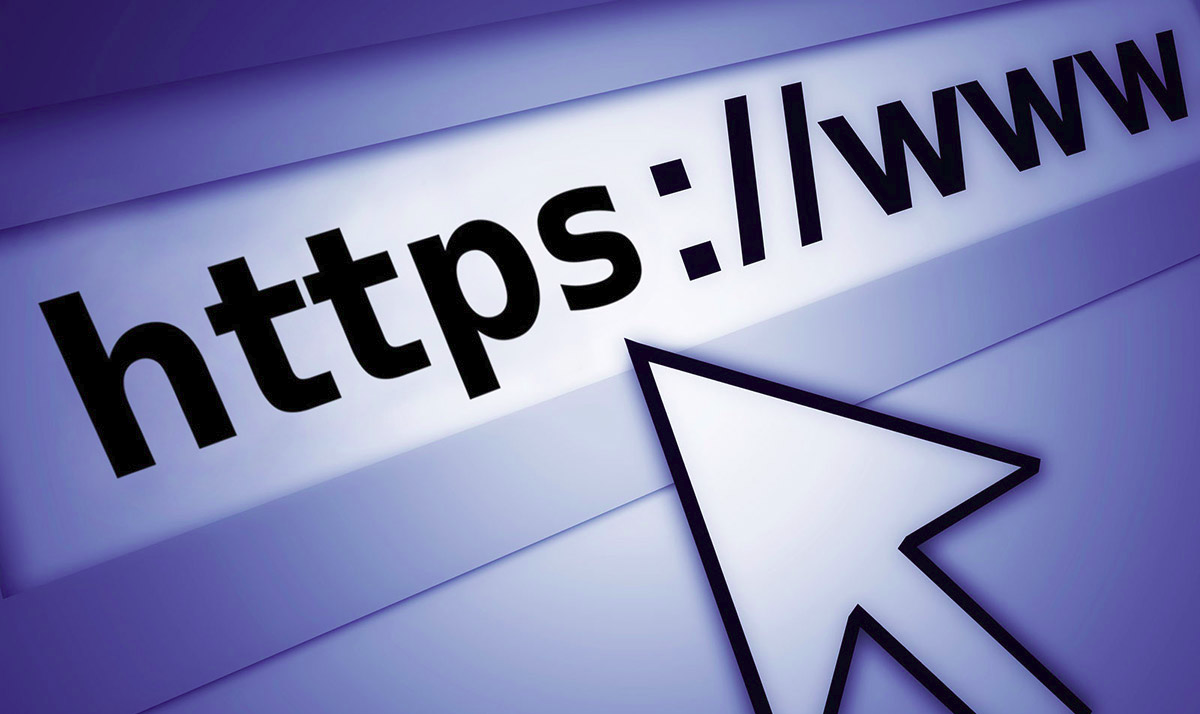
\includegraphics[height=5.5cm]{w_03_2016_Kharkevich1.png}
  
\end{figure}

HTTPS "--- это обычный HTTP, работающий через шифрованные транспортные механизмы SSL и TLS. Он обеспечивает защиту от атак, основанных на прослушивании сетевого соединения.

Глобальный переход на SSL стал трендом, и разработчики двух популярных браузеров, Mozilla Firefox\footnotemark[1] и Chromium\footnotemark[2] планируют помечать http-ресурсы как небезопасные (Non-secure).

\begin{figure}[h!]
  \centering
  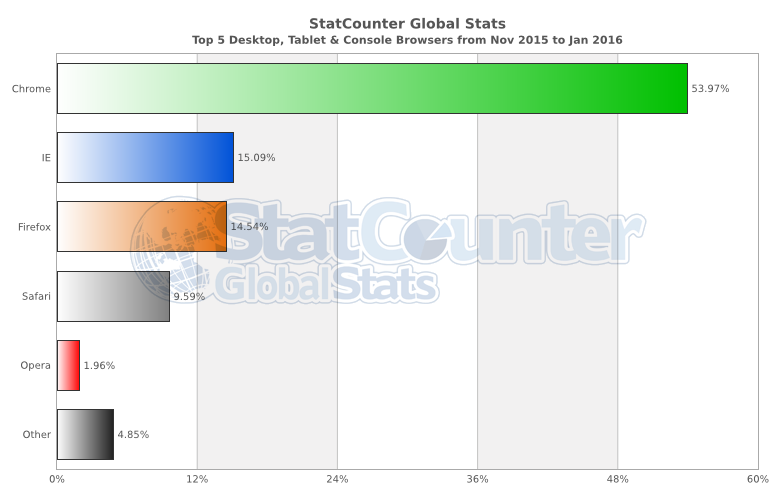
\includegraphics[height=5.5cm]{w_03_2016_Kharkevich2.png}
\caption*{StatCounter "--- статистика за 2015 год}
\end{figure}


\begin{figure}[h!]
  \centering
  
\includegraphics[width=10cm]{w_03_2016_Kharkevich3.png}
\caption*{Пример небезопаснго веб-сайта}\label{fig:Kharkevich3}
\end{figure}


При этом в Google уже с 2014 года предпочтение отдается сайтам с https\footnotemark[3].

\subsection*{Виды SSL-сертификатов}

Можно выделить следующие виды сертификатов:

\begin{itemize}
  \item Domain Validation "--- сертификат, подтверждающий только доменное имя.
  \item Organization Validation "--- сертификат, подтверждающий домен и организацию.
  \item Extended Validation "--- сертификат с расширенной проверкой.
\end{itemize}

Если Organization Validation и Extended Validation продаются только за деньги, то Domain Validation бывает и \textbf{бесплатный}.

В дальнейшем будем рассматривать только сертификаты Domain Validation.

\subsection*{Варианты получения SSL-сертификатов}

В реальной жизни для получения сертификатов существуют следующие варианты:

\begin{itemize}
  \item Самоподписанные сертификаты (self-signed-certificate) и сертификаты, подписанные собственным центром сертификации.
\begin{itemize}
  \item Из плюсов "--- возможность самостоятельно создавать \linebreak неограниченное количество SSL-сертификатов; отсутствие денежных затрат; быстрота в создании; в случае собственного удостоверяющего центра "--- доверие к данному сертификату.
  \item Из мнусов "--- необходимость добавления удостоверяющего центра в список доверенных ЦС вручную либо аналогичной процедуры для самоподписанных сертификатов; в случае использования собственного удостоверяющего центра "--- дополнительные требования по размещению и защите.
\end{itemize}


  \item Платные сертификаты от известных центров сертификации.
\begin{itemize}
  \item Из их плюсов "--- внешний гарант подлинности.
  \item Из минусов "--- нужно платить деньги.
\end{itemize}

  \item Коммерческие триальные SSL-сертификаты в качестве бесплатных.
\begin{itemize}
  \item Из их плюсов "--- бесплатность.
  \item Из минусов "--- малый срок действия и невозможность заказать повторно.
\end{itemize}

  \item Бесплатные сертификаты от StartSSL.
\begin{itemize}
  \item Из их плюсов "--- бесплатность.
  \item Из минусов "--- ручная установка сертификатов на сервер; сертификат бесплатен только для некоммерческого использования; сложности с отзывом сертификата.
\end{itemize}


  \item Бесплатные сертификаты от WoSign.
\begin{itemize}
  \item Из их плюсов "--- сертификат действительно бесплатный; у них появился англоязычный интерфейс; поддержка до пяти поддоменов в запросе на сертификат.

\begin{figure}[h!]
  \centering
  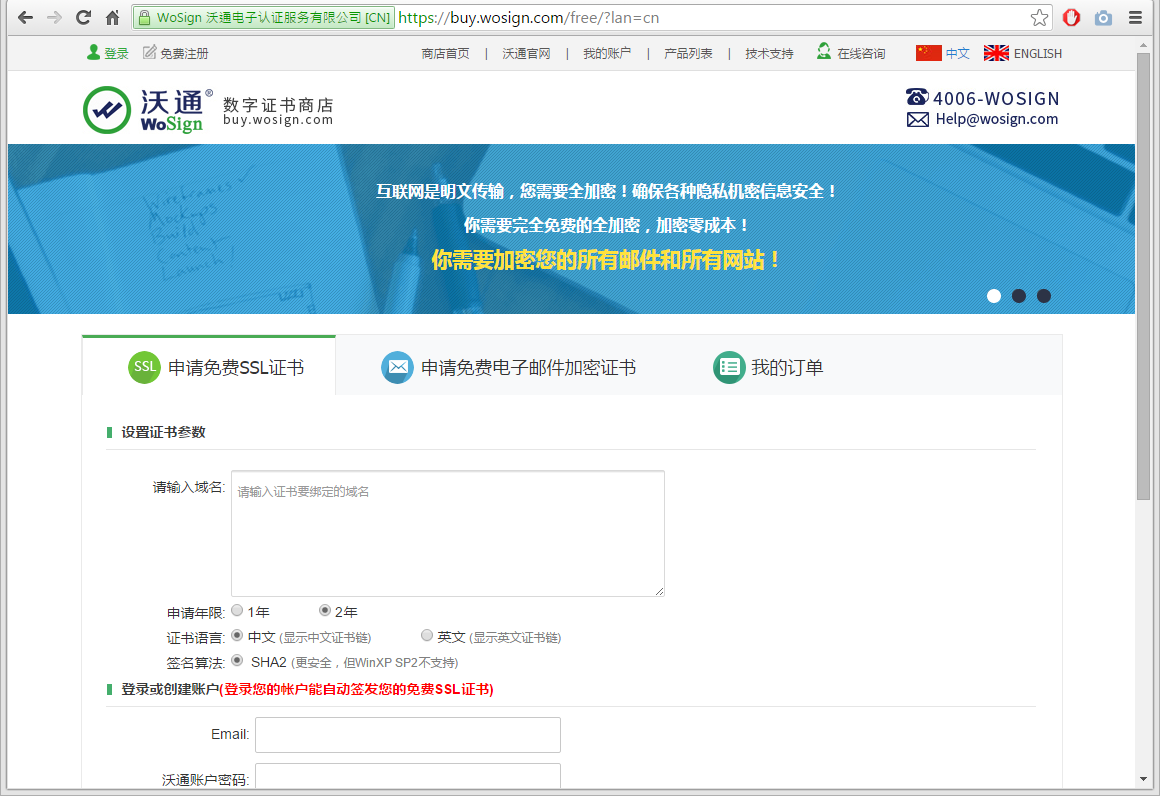
\includegraphics[height=5.5cm]{w_03_2016_Kharkevich4.png}
\caption*{WoSign на китайском языке}\label{fig:Kharkevich4}
\end{figure}

  \item Из минусов "--- ручная установка сертификатов на сервер; OCSP в Китае; для поддоменов постоянно урезаются лимиты; потенциальный MitM в связи с наличием \linebreak The Golden Shield Project.
\end{itemize}


  \item Бесплатные сертификаты от Let’s Encrypt.
\begin{itemize}
  \item Из минусов "--- новый игрок на рынке (требуется обновить списки CA); еще не вышел из бета-версии; только DV-сертификаты; есть некоторые лимиты на выпуск/перевыпуск сертификатов.
  \item Из плюсов "--- нет ограничения по применению сертификатов; может использоваться в коммерческих проектах; ACME "--- полностью автоматический процесс выдачи сертификата; срок действия сертификата до 90 дней.
\end{itemize}

\end{itemize}

\subsection*{Let’s Encrypt – наш выбор}
\begin{figure}[h!]
  \centering
  
\includegraphics[width=10cm]{w_03_2016_Kharkevich5.png}
  
\end{figure}

\subsubsection*{Шаги по установлению глобального доверия}

Для подписания пользовательских сертификатов Let’s Encrypt использует промежуточные сертификаты, которые кроме корневой подписи имеют перекрестную подпись от IdenTrust. Такая конфигурация позволила как минимум взлететь на тех браузерах, в которых еще ничего не было сказано про корневой сертификат Let’s Encrypt \footnotemark[4]

\begin{figure}[h!]
  \centering
  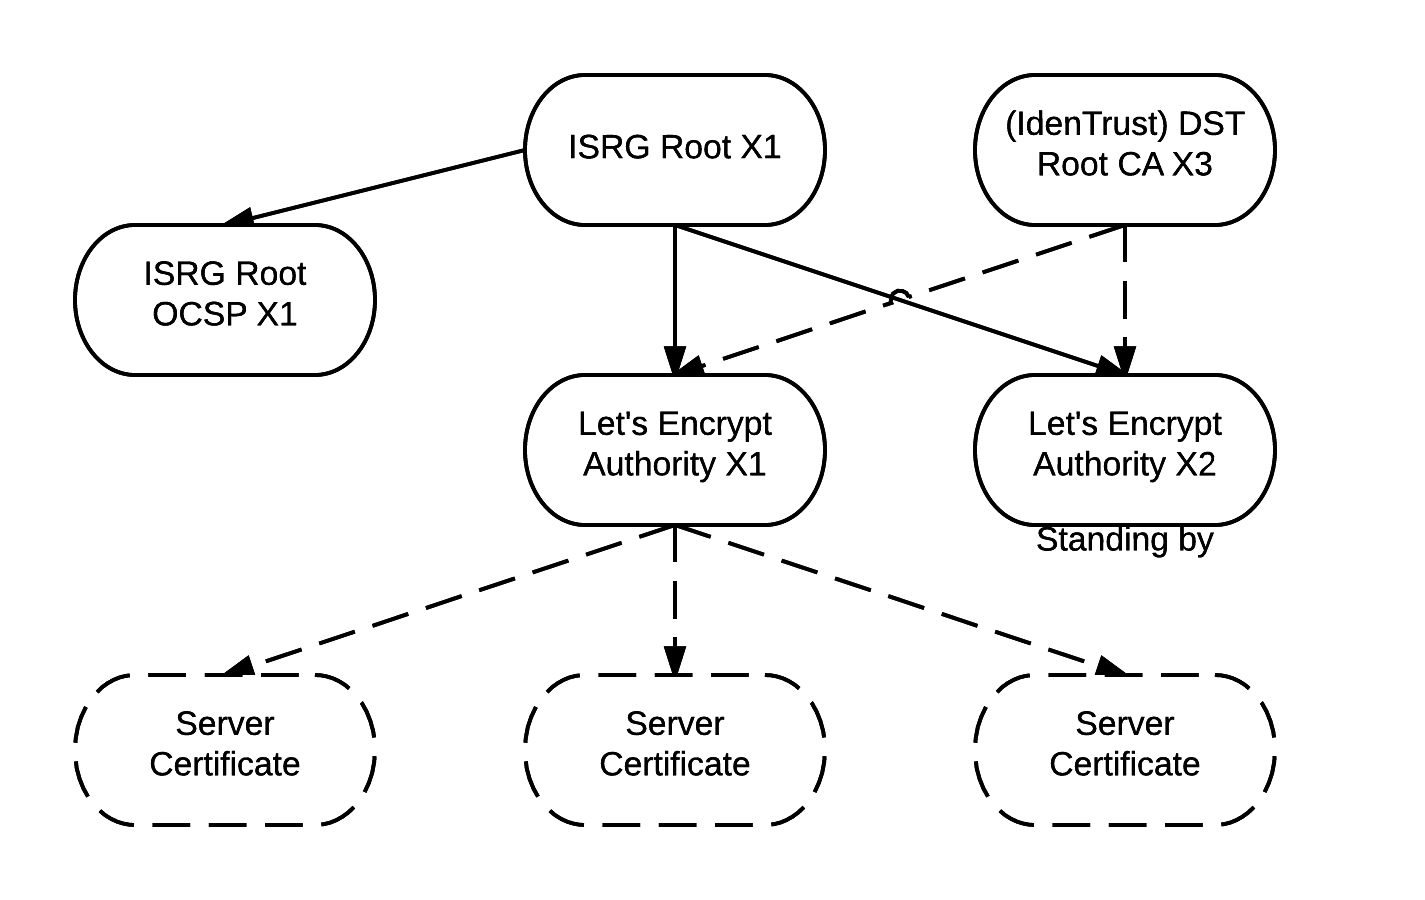
\includegraphics[height=5.5cm]{w_03_2016_Kharkevich6.png}
\caption*{Перекрестная подпись промежуточных сертификатов}\label{fig:Kharkevich6}
\end{figure}


\subsubsection*{Как работает ACME (Automatic Certificate Management Environment)}

Для получения  сертификата необходимо доказать центру сертификации, что домен, для которого пришел запрос сертификата, принадлежит запросившей сертификат стороне.

Это происходит в несколько шагов.

В первый раз взаимодействуя с Let's Encrypt CA, агент сгенерирует пару ключей, которые будет использовать для доказательства наличия прав на доменное имя.

Агент отправляет запрос в Let's Encrypt CA с указанием домена, который необходимо подтвердить.

Let’s Encrypt CA оценивает домен и выдает клиенту как минимум одну задачу на доказательство владения доменом:

\begin{itemize}
  \item Создание DNS-записи в доменной зоне для запрошенного домена.
  \item Создание ресурса, доступного по HTTP на известном URI для запрошенного домена.
\end{itemize}

Наряду с решением вышеописанной задачи, Let’s Encrypt CA  создает одноразовый ключ, который агент должен подписать своим закрытым ключом для домена, чтобы доказать, что он контролирует ключевую пару.

\begin{figure}[h!]
  \centering
  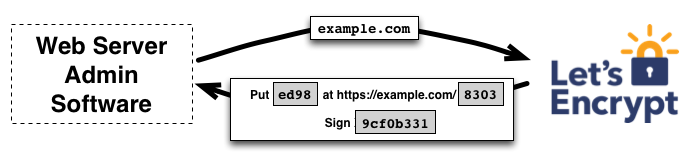
\includegraphics[width=10cm]{w_03_2016_Kharkevich7.png}
  
\end{figure}

Агент выполняет выбранную задачу и уведомляет сервер о готовности пройти валидацию.

Let’s Encrypt CA проверяет электронную цифровую подпись и доступность файлов или записей в DNS.

В случае, если цифровая подпись верна и выбранная задача решена верно, Let’s Encrypt CA считает, что агент имеет право на управление сертификатами для запрошенного домена.

Ключевая пара, использованная агентом, становится <<авторизованной парой ключей>> для запрошенного домена.

\begin{figure}[h!]
  \centering
  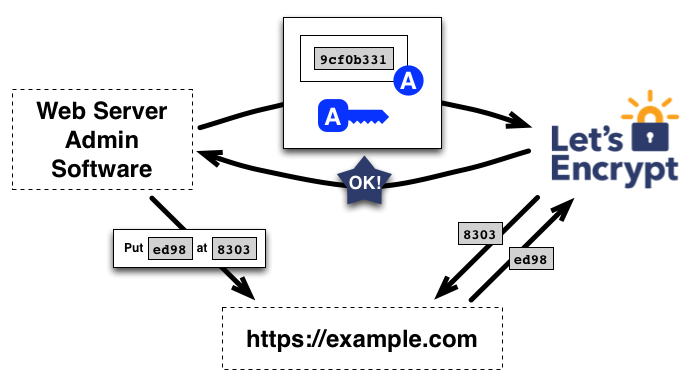
\includegraphics[height=5.5cm]{w_03_2016_Kharkevich8.png}
\caption*{Успешное выполнение всех задач от Let’s Encrypt}\label{fig:Kharkevich8}
\end{figure}


После авторизации агент может запросить, обновить или отозвать сертификаты для своего домена. Сообщения должны быть подписаны авторизованной парой ключей.

\begin{figure}[h!]
  \centering
  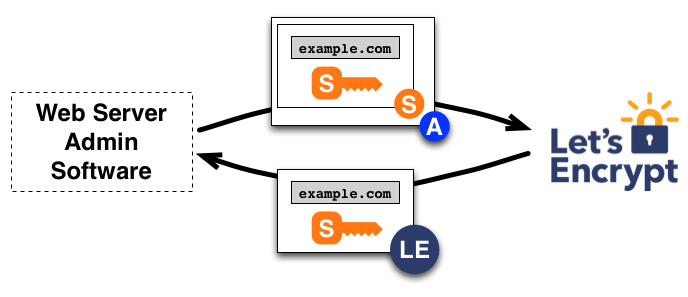
\includegraphics[width=10cm]{w_03_2016_Kharkevich9.png}
\caption*{Выпуск сертификата}\label{fig:Kharkevich9}
\end{figure}

\begin{figure}[h!]
  \centering
  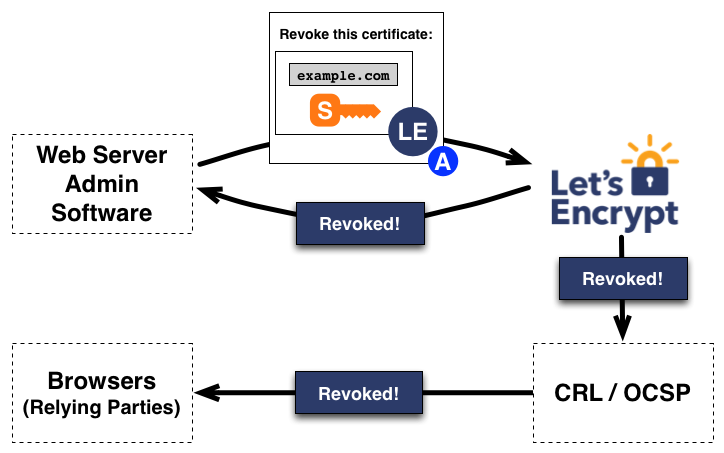
\includegraphics[height=5.5cm]{w_03_2016_Kharkevich10.png}
\caption*{Отзыв сертификата}\label{fig:Kharkevich10}
\end{figure}


\subsubsection*{Клиенты/плагины для Let's Encrypt}

Для Let’s Encrypt существует как официальная реализация клиентской части, так и множество других реализаций протокола \linebreak ACME (написаны на Python, Go, C\#, Ruby, Bash).

Официальный клиент поддерживает расширение функциональности за счет плагинов. На текущий момент, реализованные плагины представлены на странице github \footnotemark[5].

Написать свой плагин достаточно просто: нужно всег лишь прочитать документацию \footnotemark[6] и написать его.

\subsection*{Примеры из реальной жизни и немного статистики}

Судя по crt.sh "--- Let's Encrypt выпустил громадное количество сертификатов и с отрывом лидирует над остальными.

\begin{figure}[h!]
  \centering
  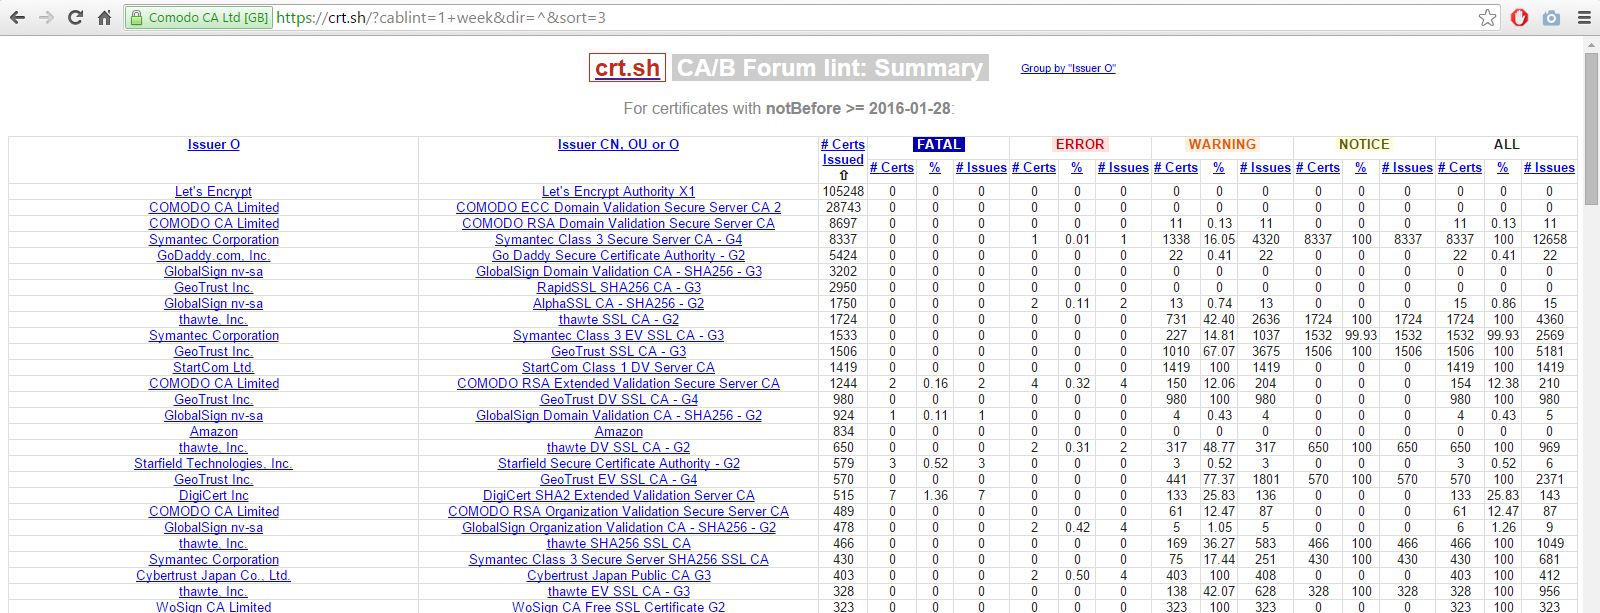
\includegraphics[width=10cm]{w_03_2016_Kharkevich11.png}
\caption*{Статистика по версии от crt.sh}\label{fig:Kharkevich11}
\end{figure}


\subsubsection*{Забытые обновления сертификатов}

В заключение "--- несколько случаев пропущенных обновлений сертификатов:

\begin{itemize}
  \item Ростелеком в 2010 году \footnotemark[7]
  \item Хабр и habrastorage.org в 2014 году \footnotemark[8]

\begin{figure}[h!]
  \centering
  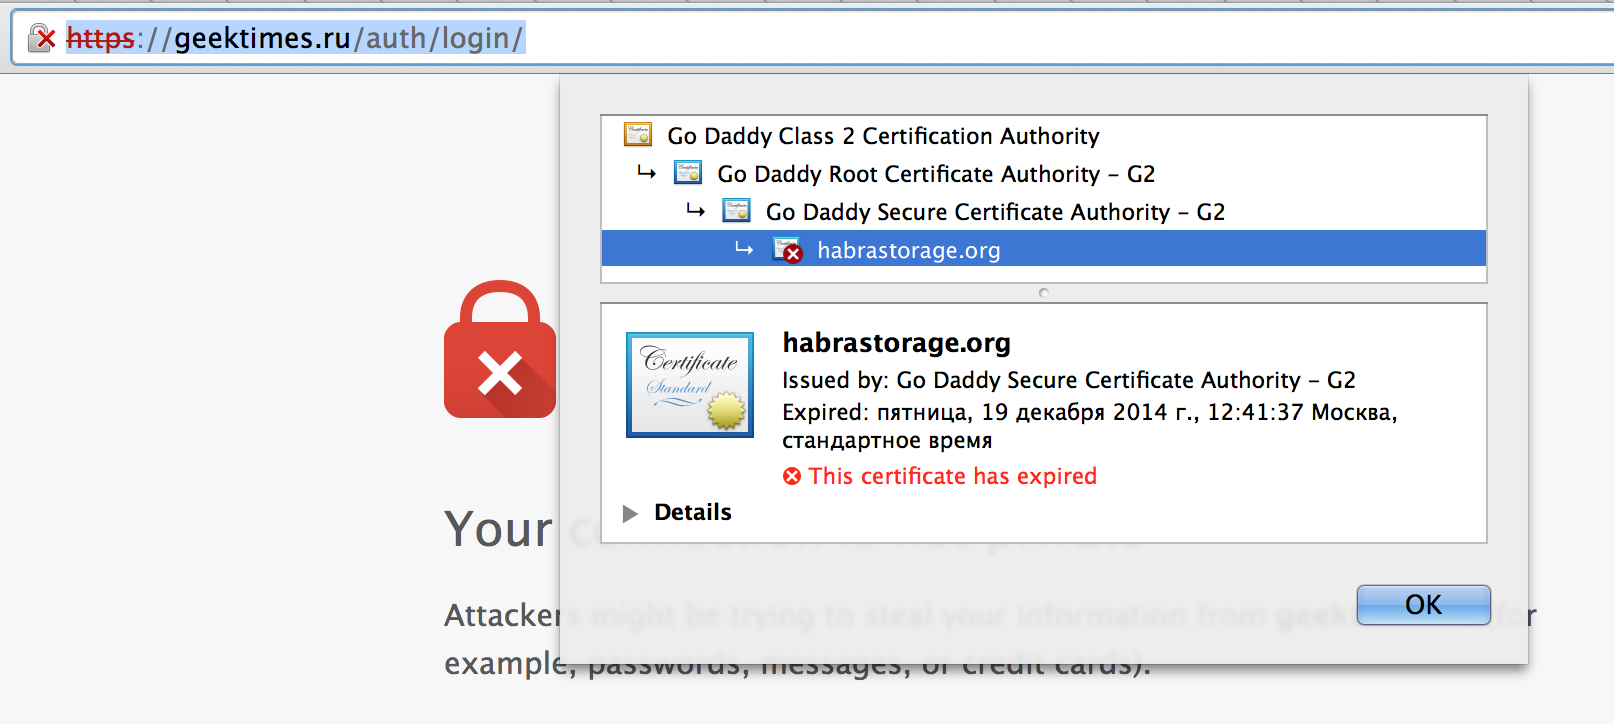
\includegraphics[width=10cm]{w_03_2016_Kharkevich12.png}
  
\end{figure}

  \item RU-CENTER (ssl.ru) в 2016 году

\begin{figure}[h!]
  \centering
  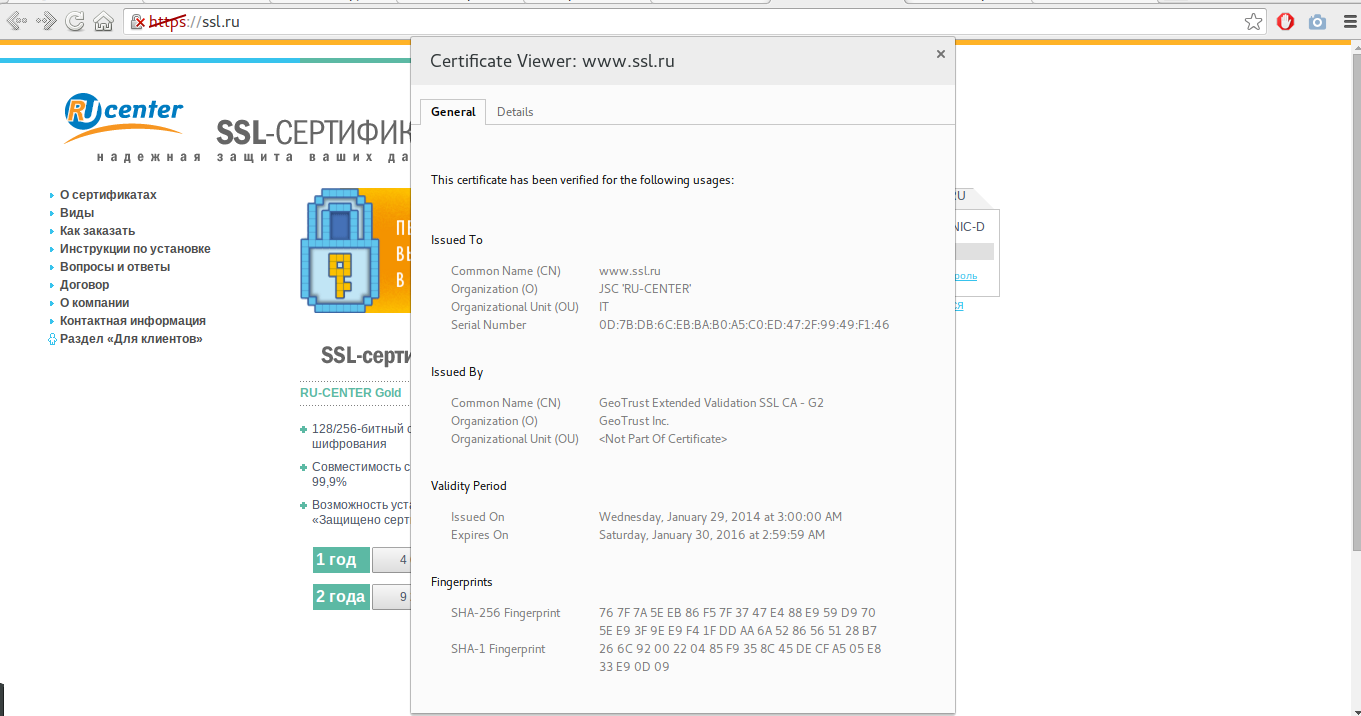
\includegraphics[height=5.5cm]{w_03_2016_Kharkevich13.png}
  
\end{figure}

\end{itemize}

\begin{thebibliography}{99}
\bibitem{Kharkevich1} Mozilla Security Blog: Deprecating Non-Secure HTTP. \url{https://blog.mozilla.org/security/2015/04/30/deprecating-non-secure-http/} {}
\bibitem{Kharkevich2}The Chromium Projects proposal: Marking HTTP As Non-Secure. \url{https://www.chromium.org/Home/chromium-security/marking-http-as-non-secure}{}
\bibitem{Kharkevich3}Google Webmaster Central Blog: HTTPS as a ranking signal. \url{https://googlewebmastercentral.blogspot.com.by/2014/08/https-as-ranking-signal.html}{}
\bibitem{Kharkevich4}Let’s Encrypt certificates. \url{https://letsencrypt.org/certificates/}{}
\bibitem{Kharkevich5}Letsencrypt officially supported plugins. \url{https://github.com/letsencrypt/letsencrypt/wiki/Plugins}{}
\bibitem{Kharkevich6}Writing your own letsencrypt plugin. \url{https://letsencrypt.readthedocs.org/en/latest/contributing.html#dev-plugin}{}
\bibitem{Kharkevich7}Geektimes: Ростелеком забыл обновить ssl-сертификат gosuslugi.ru. \url{https://geektimes.ru/post/102984/}{}
\bibitem{Kharkevich8}Geektimes: Пора обновить сертификат на Habrastorage.org. \url{https://geektimes.ru/post/243231/}
\bibitem{Kharkevich9}Поиск по сертификатам. \url{https://crt.sh/}{}
\bibitem{Kharkevich10}Тестирование конфигурации SSL. \url{https://www.ssllabs.com/ssltest/}
\bibitem{Kharkevich11}Генератор SSL конфигурационных файлов от Mozilla. \url{https://mozilla.github.io/server-side-tls/ssl-config-generator/}{}
\bibitem{Kharkevich12}Анализ веб-трафика. \url{http://gs.statcounter.com/}{}
\bibitem{Kharkevich13}Let's Encrypt how it works. \url{https://letsencrypt.org/howitworks/technology/}{}
\end{thebibliography}
\end{document}
